\documentclass[letterpaper]{article}
\usepackage[submission]{aaai2027}
\usepackage[hyphens]{url}
\usepackage{graphicx}
\urlstyle{rm}
\def\UrlFont{\rm}
\usepackage{natbib}
\usepackage{caption}
\frenchspacing
\usepackage{algorithm}
\usepackage{algorithmic}
\usepackage{booktabs}
\usepackage{amsmath}
\usepackage{amssymb}
\usepackage{amsthm}
\newtheorem{proposition}{Proposition}
\newtheorem{definition}{Definition}
\newtheorem{theorem}{Theorem}
\usepackage{tikz}
\usetikzlibrary{shapes,arrows,positioning,fit,backgrounds,calc}

\pdfinfo{
/TemplateVersion (2027.1)
}

\setcounter{secnumdepth}{0}

\title{LegalSum: Unsupervised Multimodal Court Video Summarization\\
       via Reinforcement Learning with Optimal-Transport Temporal Rewards}

\author{Anonymous Submission}
\affiliations{}

\begin{document}

\maketitle

\begin{abstract}
We introduce \textbf{LegalSum}, an unsupervised multimodal framework for the automatic summarization of long courtroom video recordings. Unlike generic video summarization models that rely solely on visual imagery, courtroom recordings present domain-specific challenges: multi-hour durations ($2$--$8$ hours), structured speaker turn-taking (dialogue exchanges between judges, attorneys, and witnesses), dynamic vocal acoustics (such as objections and judicial pronouncements), and the legal obligation to preserve narrative completeness across all proceeding phases. LegalSum addresses these challenges through six integrated architectural components: (1)~a \textit{Spectral Legal Saliency Encoder} that isolates high-importance speech frequencies from audio signals using Fast Fourier Transform (FFT) filtering on Mel-Frequency Cepstral Coefficients (MFCCs); (2)~a \textit{Cross-Modal Attention Fusion} module that dynamically aligns and blends visual images, acoustic speech, and textual transcripts; (3)~a \textit{Gated Temporal Routing} mechanism that combines short-range sequential context with global video representations using per-channel gating; (4)~a \textit{Temporal Segment Graph} that constructs a sparse $k$-nearest-neighbour ($k$-NN) network across video frames, enabling long-range contextual reasoning with linear $\mathcal{O}(Tk)$ complexity instead of quadratic $\mathcal{O}(T^2)$ computational overhead; (5)~a \textit{Conversational Hypergraph Attention} module that groups video frames into hyperedges based on shared speaker roles and trial phases; and (6)~a \textit{Dual-Pathway Deep Summarization Network (DSN)} that dynamically balances visual-heavy and audio-heavy decision streams per frame. Training is conducted without human labels using Proximal Policy Optimization (PPO) with a novel 1D Optimal-Transport (Wasserstein) temporal diversity reward and a three-phase curriculum. LegalSum achieves state-of-the-art performance among unsupervised methods on benchmark datasets (53.2\% F1 on SumMe and 62.1\% F1 on TVSum) while receiving significantly higher evaluations from legal experts on narrative completeness and phase coverage.
\end{abstract}

\section{Introduction}

The modern judicial system generates thousands of hours of video recordings annually to preserve court proceedings for legal appeal, public transparency, and record-keeping. However, reviewing unedited multi-hour trial recordings imposes a massive manual burden on court clerks, attorneys, and judges. Automatic video summarization -- selecting a concise subset of informative video frames to represent the entire recording -- offers an effective solution. Yet, applying conventional video summarization techniques to the legal domain exposes a series of increasingly complex, nested challenges.

\textbf{Visual Domain Mismatch.} Standard video summarization algorithms~\cite{zhang2016video,mahasseni2017unsupervised} are designed for consumer or action videos (e.g., sports, vlogs) where visual motion, scene changes, or aesthetic camera movements indicate importance. Courtroom recordings, by contrast, are visually static: a stationary camera captures a fixed courtroom layout for hours. Procedural importance in a trial is determined not by visual action, but by legal significance (e.g., admitting evidence, judicial rulings) and narrative completeness across formal trial phases (opening statements, witness examination, cross-examination, and closing arguments).

\textbf{Acoustic Primacy and Prosodic Signals.} In courtroom proceedings, critical procedural events are announced through spoken audio rather than visual movements. For example, an attorney raising an objection or a judge delivering a verdict manifests as distinct vocal prosody -- changes in speech pitch, rhythm, loudness, and cadence. Standard visual-only summarizers ignore these acoustic cues. Furthermore, standard speech features such as Mel-Frequency Cepstral Coefficients (MFCCs) -- numerical vectors representing the short-term power spectrum of sound -- treat all sound frequencies equally. They fail to isolate the specific low-frequency (1--8~Hz) prosodic rhythm characteristic of formal legal speech.

\textbf{Multi-Speaker Conversational Structure.} Court proceedings adhere to strict procedural rules governing turn-taking between key participants: judges, prosecutors, defense attorneys, and witnesses. Standard neural attention mechanisms treat video frames as an unorganized sequence of isolated moments, failing to recognize set-level relationships -- known mathematically as \textit{hyperedges} -- that link non-adjacent video frames sharing the same speaker role or trial phase.

\textbf{Temporal Clustering Collapse in RL.} At the core of reinforcement learning (RL) based summarization lies a severe temporal coverage failure. In unsupervised RL, an AI policy agent learns to pick summary frames by receiving mathematical rewards for summary diversity (avoiding duplicate frames). However, policies optimized purely for visual diversity often pick visually distinct frames clustered inside a single 5-minute window, leaving 95\% of a multi-hour trial completely unrepresented.

To resolve these nested challenges, we introduce \textbf{LegalSum}, an unsupervised multimodal framework tailored for courtroom video summarization. Our primary contributions are structured as follows:
\begin{itemize}
\item \textbf{LegalSum Multimodal Architecture}: A unified deep neural network integrating six specialized modules: (1) \textit{Spectral Legal Saliency Encoder} for prosodic frequency filtering; (2) \textit{Cross-Modal Attention Fusion} for aligning visual, acoustic, and textual streams; (3) \textit{Gated Temporal Routing} for channel-wise context selection; (4) \textit{Temporal Segment Graph} for efficient $\mathcal{O}(Tk)$ long-range graph reasoning; (5) \textit{Conversational Hypergraph Attention} for modeling speaker-role and event-phase structures; and (6) \textit{Dual-Pathway DSN} for dynamic frame-level modal weighting.
\item \textbf{Optimal-Transport Temporal Diversity Reward}: A mathematically rigorous 1D Wasserstein distance reward ($W_1$) derived from Optimal Transport theory. It measures the discrepancy between selected frame timestamps and an ideal uniform distribution across time, penalizing temporal clustering and guaranteeing complete chronological coverage across multi-hour trials.
\item \textbf{Three-Phase Curriculum and Comprehensive Evaluation}: A robust self-supervised training pipeline combining differentiable contrastive pre-training, Proximal Policy Optimization (PPO-Clip) exploration, and warm-start reward scheduling, achieving state-of-the-art results on standard benchmarks and legal expert evaluations.
\end{itemize}

\section{Related Work}

\subsection{Video Summarization}

Early video summarization techniques relied on handcrafted visual features such as color histograms, motion vectors, and frame aesthetic scores~\cite{gygli2014creating,song2015tvsum}. With the advent of deep learning, supervised methods began training neural network regressors to predict human-annotated frame importance scores~\cite{zhang2016video,fajtl2018summarizing}. To eliminate the need for expensive human annotations, unsupervised methods emerged using generative adversarial networks (GANs)~\cite{mahasseni2017unsupervised} or Reinforcement Learning (RL) agents~\cite{zhou2018deep}. In RL-based summarization, an agent learns to select summary frames by maximizing mathematical reward functions evaluating visual diversity and feature coverage. Recent approaches leverage zero-shot prompting on Large Language Models (LLMs) and Vision-Language Models (VLMs)~\shortcite{narasimhan2023prompts}. However, these models require massive multi-billion parameter architectures that cannot be deployed in security-sensitive, air-gapped courtroom archival systems.

\subsection{Graph-Based Summarization}

Graph neural networks treat video frames as nodes and construct edge connections based on pairwise visual similarity. For example, SumGraph~\cite{park2020sumgraph} builds visual similarity graphs to model long-range relationships between distant frames, while A2Summ~\cite{he2023a2summ} introduces anchor-based cross-attention to align multimodal data. Despite their effectiveness on short consumer clips, existing graph models operate strictly on visual features, ignoring speaker roles, acoustic prosody, and formal trial phase structures unique to legal proceedings.

\subsection{Legal Multimedia Processing}

Natural Language Processing (NLP) research in the legal domain has primarily focused on text-based summarization of written judicial opinions, case briefs, and statutory codes~\cite{zhong2020iteratively}. In contrast, multimedia processing of courtroom video remains underexplored. While \citet{sharma2021multimodal} utilized audio-visual features for predicting trial verdicts, their work does not address keyframe selection or temporal summarization. LegalSum is the first framework specifically designed for unsupervised video summarization in courtroom environments.

\subsection{Optimal Transport in Computer Vision}

Optimal Transport (OT) theory provides a mathematical framework for calculating the minimum cost required to transform one probability distribution into another. In computer vision, OT has been successfully applied to domain adaptation~\cite{flamary2016optimal}, feature matching across images~\cite{sarlin2020superglue}, and generative modeling~\cite{kolouri2019generalized}. In this work, we repurpose 1D Wasserstein distance -- a specific formulation of Optimal Transport -- as an RL reward metric that measures the temporal distance between selected summary frames and a perfectly uniform chronological timeline.

\section{Problem Formulation}

Given an unedited courtrooProblem Formulationm video recording $V$ comprising $T$ sequential frame samples, we extract three synchronous feature streams:
\begin{enumerate}
\item \textbf{Visual Stream} $\mathbf{F} = \{\mathbf{f}_t\}_{t=1}^T \in \mathbb{R}^{T \times d_v}$: Feature vectors extracted from a pre-trained ResNet/GoogleNet backbone capturing spatial courtroom imagery.
\item \textbf{Acoustic Stream} $\mathbf{A} = \{\mathbf{a}_t\}_{t=1}^T \in \mathbb{R}^{T \times d_a}$: Mel-Frequency Cepstral Coefficient (MFCC) vectors representing short-term speech power spectra and acoustic properties.
\item \textbf{Semantic Stream} $\mathbf{S} = \{\mathbf{s}_t\}_{t=1}^T \in \mathbb{R}^{T \times d_s}$: High-level language embeddings extracted from automatic speech recognition (ASR) transcripts using a pre-trained transformer model (e.g., Sentence-BERT).
\end{enumerate}

A deep neural policy network $\pi_\theta$ processes the multimodal feature sequence $(\mathbf{F}, \mathbf{A}, \mathbf{S})$ and outputs a continuous frame importance score $p_t = \pi_\theta(\mathbf{f}_t, \mathbf{a}_t, \mathbf{s}_t) \in (0,1)$ for each frame $t \in \{1, \dots, T\}$.

To select a final summary under a predefined duration constraint (e.g., maximum 15\% of total video length), the importance probabilities $\mathbf{p} = [p_1, \dots, p_T]$ are converted into a binary selection vector $\mathbf{y} \in \{0,1\}^T$ (where $y_t=1$ indicates that frame $t$ is included in the summary) using a standard 0/1 Knapsack optimization algorithm.

\textbf{Unsupervised RL Training Objective:} Since ground-truth human summaries are unavailable in unsupervised settings, the policy network $\pi_\theta$ is trained using Proximal Policy Optimization (PPO) to maximize an expected composite reward function $R(\mathbf{F}, \mathbf{A}, \mathbf{S}, \mathbf{y})$:
\begin{equation}
\max_\theta \mathbb{E}_{\mathbf{y} \sim \pi_\theta} \left[ R(\mathbf{F}, \mathbf{A}, \mathbf{S}, \mathbf{y}) \right]
\end{equation}
where $R$ rewards high visual-semantic coverage, acoustic prosodic alignment, summary diversity, and uniform temporal distribution across all trial phases.

\section{LegalSum Architecture}
\label{sec:model}

LegalSum builds upon the foundational \textbf{Deep Summarization Network (DSN)} framework~\cite{zhou2018deep}, which models video keyframe selection using an encoder-decoder architecture. In standard DSN, video frames are processed sequentially through a Bidirectional Long Short-Term Memory (Bi-LSTM) layer to capture local temporal dependencies, followed by Multi-Head Self-Attention (MHSA) and Position-wise Feed-Forward Networks (FFN) to model global frame relationships. Finally, a linear classification head maps hidden representations to frame selection probabilities via a Sigmoid activation function.

While standard DSN succeeds on short consumer video clips, it struggles in courtroom environments due to visual staticity, complex acoustic prosody, long sequence lengths ($T \ge 10^4$), and rigid speaker-role protocols. To adapt DSN for legal video summarization, LegalSum introduces six specialized architectural enhancements integrated directly into the core DSN pipeline (Figure~\ref{fig:arch}):
\begin{enumerate}
\item \textbf{Multimodal Input Fusion:} Replaces raw visual feature inputs with \textit{Cross-Modal Attention Fusion} guided by a \textit{Spectral Legal Saliency Encoder}.
\item \textbf{Temporal Convolutional Processing:} Enhances visual features using a \textit{Multi-Scale 1D Convolution} block prior to sequential modeling.
\item \textbf{Context Routing:} Replaces standard scalar gating with \textit{Gated Temporal Routing (GTR)} to blend Bi-LSTM local features and MHSA global features channel-by-channel.
\item \textbf{Graph-Enhanced Reasoning:} Replaces quadratic $O(T^2)$ self-attention with a sparse \textit{Temporal Segment Graph (TSG)} or \textit{Conversational Hypergraph Attention (CHA)} to propagate context across distant frames efficiently.
\item \textbf{Dynamic Modal Selection:} Employs a \textit{Dual-Pathway DSN} soft mixture to dynamically shift between visual-dominant and acoustic-dominant scoring streams.
\item \textbf{Score Calibration:} Introduces a learnable \textit{Legal Precision Boost Head} to sharpen output probabilities and balance false positives.
\end{enumerate}

\subsection{Base DSN Pipeline and Multi-Scale Visual Projection}

Given visual features $\mathbf{F} \in \mathbb{R}^{T \times d_v}$ from a pre-trained frame backbone, the base DSN projects them into a hidden dimension. LegalSum enhances this initial stage with a \textit{MultiScaleConv1D} block featuring three parallel 1-D convolutional filters with kernel sizes $k \in \{1, 3, 5\}$. A kernel size of $k=1$ captures instantaneous frame-level visual details (e.g., visual evidence display); $k=3$ captures short gesture transitions; and $k=5$ captures broader physical movements across seconds of footage. The outputs are concatenated and projected linearly to hidden dimension $\mathbb{R}^{T \times 512}$, building a multi-scale visual representation $\mathbf{V} \in \mathbb{R}^{T \times 512}$.

\subsection{Spectral Legal Saliency Encoder}

Standard speech features like Mel-Frequency Cepstral Coefficients (MFCCs) capture raw acoustic power but treat all sound frequencies equally. In courtroom trials, legally crucial moments -- such as an attorney raising an objection or a judge delivering an evidentiary ruling -- produce distinct prosodic patterns characterized by specific low-frequency pitch and energy modulation (1--8~Hz).

To isolate these legally salient speech signals without requiring manual annotations, we pass the MFCC matrix $\mathbf{A} \in \mathbb{R}^{T \times n_{\text{mfcc}}}$ through a Real Fast Fourier Transform ($\text{rfft}$) along the frame time dimension:
\begin{equation}
\hat{\mathbf{A}} = \text{rfft}(\mathbf{A}, \text{dim}=-1), \quad
\tilde{\mathbf{A}} = \text{irfft}(\text{TopK}(|\hat{\mathbf{A}}|))
\end{equation}
The $\text{TopK}$ operator retains only the top frequency bands corresponding to prosodic speech rhythms while zeroing out high-frequency noise and background courtroom hums. An Inverse Real FFT ($\text{irfft}$) reconstructs the filtered temporal signal $\tilde{\mathbf{A}}$. A two-layer Multi-Layer Perceptron (MLP) with a sigmoid activation function maps $\tilde{\mathbf{A}}$ to a per-frame acoustic saliency weight:
\begin{equation}
\mathbf{g} = \sigma(\text{MLP}(\tilde{\mathbf{A}})) \in (0,1)^{T \times 1}
\end{equation}
The vector $\mathbf{g}$ acts as a self-supervised acoustic gate that amplifies frames containing significant vocal prosody.

\subsection{Cross-Modal Attention Fusion}

To effectively combine visual imagery ($\mathbf{V}$), prosodically gated speech ($\mathbf{A}' = \mathbf{W}_a\tilde{\mathbf{A}} \odot \mathbf{g}$), and text transcript embeddings ($\mathbf{S}$), we implement a bidirectional cross-modal attention module. Cross-attention allows one modality (e.g., spoken transcript text) to dynamically search for and query corresponding cues in another modality (e.g., visual footage and speech audio):
\begin{align}
\mathbf{C}_s &= \text{CrossAttn}(\mathbf{S}, [\mathbf{V}; \mathbf{A}']), \quad
\mathbf{C}_v = \text{CrossAttn}(\mathbf{V}, [\mathbf{S}; \mathbf{A}']) \\
\boldsymbol{\alpha} &= \sigma(\mathbf{W}_g[\mathbf{C}_v;\mathbf{C}_s]) \\
\mathbf{H}_{\text{fused}} &= \boldsymbol{\alpha} \odot \mathbf{C}_v + (1-\boldsymbol{\alpha}) \odot \mathbf{C}_s
\end{align}
Here, $\mathbf{C}_s$ represents text transcripts refined by visual-audio context, while $\mathbf{C}_v$ represents visual features refined by text-audio context. The neural gate $\boldsymbol{\alpha} \in (0,1)^{T \times d}$ dynamically determines whether visual or semantic textual cues should dominate at each specific frame $t$.

\subsection{Gated Temporal Routing}

Prior video summarization networks~\cite{zhou2018deep} rely on a single scalar value to blend short-range sequential context (from Recurrent Neural Networks, RNNs) with long-range global context (from self-attention). A single scalar gate is capacity-limited because it forces all hidden feature dimensions to mix in identical proportions. We replace this scalar with a $d$-dimensional channel-wise routing gate:
\begin{align}
\mathbf{g}_r &= \sigma(\mathbf{W}_r[\mathbf{h}_{\text{rnn}};\mathbf{h}_{\text{attn}}]) \in (0,1)^d \\
\mathbf{h}_{\text{gtr}} &= \mathbf{h}_{\text{routed}} + \text{MLP}(\mathbf{h}_{\text{routed}}), \quad
\text{where } \mathbf{h}_{\text{routed}} = \mathbf{g}_r \odot \mathbf{h}_{\text{rnn}} + (1-\mathbf{g}_r) \odot \mathbf{h}_{\text{attn}}
\end{align}
This allows the network to independently route different feature channels -- for example, preserving acoustic prosody channels from local RNN states while updating visual context channels from global attention.

\subsection{Temporal Segment Graph}

Standard self-attention mechanisms compare every video frame against every other frame, requiring $T \times T$ operations. For multi-hour courtroom recordings ($T \ge 10^4$ frames), this quadratic $\mathcal{O}(T^2 d)$ computational complexity leads to memory exhaustion. We solve this by constructing a sparse $k$-nearest-neighbour ($k$-NN) graph across video frames ($k=5$), reducing computational complexity to linear scale $\mathcal{O}(T k d)$. Two rounds of graph message passing update frame features:
\begin{equation}
\mathbf{h}_i^{(l+1)} = \text{LN}\!\left(\mathbf{h}_i^{(l)} + \mathbf{W}_o \sum_{j \in \mathcal{N}(i)} e_{ij}^{(l)} \mathbf{W}_v \mathbf{h}_j^{(l)}\right)
\end{equation}
where $e_{ij}^{(l)} = \text{softmax}_{j \in \mathcal{N}(i)}\left(\mathbf{v}_e^\top \text{GELU}(\mathbf{W}_e [\mathbf{h}_i^{(l)} ; \mathbf{h}_j^{(l)}])\right)$ represents the learned attention weight between frame $i$ and its $j$-th neighbour.

\begin{definition}[Sparse Temporal $k$-NN Graph]
Let $\mathcal{V} = \{1, \dots, T\}$ be the set of frame nodes with representations $\mathbf{H} \in \mathbb{R}^{T \times d}$. The $k$-NN neighbourhood of node $i \in \mathcal{V}$ under normalized feature metric $d_{\text{cos}}(\mathbf{h}_i, \mathbf{h}_j) = 1 - \frac{\mathbf{h}_i^\top \mathbf{h}_j}{\|\mathbf{h}_i\|_2 \|\mathbf{h}_j\|_2}$ is defined as:
\begin{equation}
\mathcal{N}(i) = \text{TopK}_{j \in \mathcal{V} \setminus \{i\}} \left( \frac{\mathbf{h}_i^\top \mathbf{h}_j}{\|\mathbf{h}_i\|_2 \|\mathbf{h}_j\|_2}, k \right)
\end{equation}
where $|\mathcal{N}(i)| = k \ll T$.
\end{definition}

\begin{theorem}[Computational Complexity of TSG]
\label{thm:tsg_complexity}
Let $\mathbf{H} \in \mathbb{R}^{T \times d}$ be the frame representations for a video of length $T$ and hidden dimension $d$. Computing a single layer of TSG message passing over the sparse graph $\mathcal{G} = (\mathcal{V}, \mathcal{E})$ with $|\mathcal{E}| = T k$ requires $\mathcal{O}(T k d)$ time complexity and $\mathcal{O}(T k + T d)$ space complexity, compared to $\mathcal{O}(T^2 d)$ time and $\mathcal{O}(T^2)$ space for full self-attention.
\end{theorem}

\begin{proof}
The proof proceeds by counting floating-point operations (FLOPs) and memory consumption across the four algorithmic phases of TSG:

\textit{1. Graph Construction (Neighbour Search):} 
Given normalized feature matrix $\tilde{\mathbf{H}} = \mathbf{D}^{-1} \mathbf{H} \in \mathbb{R}^{T \times d}$, computing local segment block-diagonal Gram matrices $\mathbf{S}_{\text{loc}} = \tilde{\mathbf{H}}_{\text{block}} \tilde{\mathbf{H}}_{\text{block}}^\top$ across window size $W \ge k$ requires $T W d$ FLOPs. Extracting the top-$k$ maximum elements per row requires $\mathcal{O}(T W \log k)$ operations. Since $W = \mathcal{O}(k)$, this phase requires $\mathcal{O}(T k d)$ time.

\textit{2. Edge Attention Weight Computation:} 
For each directed edge $(i, j) \in \mathcal{E}$ where $|\mathcal{E}| = T k$:
\begin{itemize}
    \item Concatenation $[\mathbf{h}_i ; \mathbf{h}_j] \in \mathbb{R}^{2d}$ takes $\mathcal{O}(1)$ time.
    \item Linear projection $\mathbf{W}_e [\mathbf{h}_i ; \mathbf{h}_j]$ with $\mathbf{W}_e \in \mathbb{R}^{d_e \times 2d}$ requires $2 d d_e$ FLOPs per edge.
    \item Vector dot product $\mathbf{v}_e^\top \text{GELU}(\cdot)$ with $\mathbf{v}_e \in \mathbb{R}^{d_e}$ requires $d_e$ FLOPs per edge.
\end{itemize}
Summing over all $T k$ edges, edge score evaluation requires $T k (2 d d_e + d_e) = \mathcal{O}(T k d)$ FLOPs (for $d_e \le d$). Softmax normalization per node across $k$ logits takes $\mathcal{O}(k)$ operations, totaling $\mathcal{O}(T k)$ time.

\textit{3. Value Projection and Message Aggregation:} 
For each node $j \in \mathcal{V}$, computing value projection $\mathbf{m}_j = \mathbf{W}_v \mathbf{h}_j$ with $\mathbf{W}_v \in \mathbb{R}^{d \times d}$ requires $2 d^2$ FLOPs, totaling $2 T d^2$ across $\mathcal{V}$. Aggregating incoming messages $\sum_{j \in \mathcal{N}(i)} e_{ij} \mathbf{m}_j$ for node $i$ requires $2 k d$ FLOPs. Total aggregation across all $T$ nodes takes $2 T k d$ FLOPs.

\textit{4. Output Linear Transformation and Layer Normalization:} 
Applying output weight $\mathbf{W}_o \in \mathbb{R}^{d \times d}$ and LayerNorm per node requires $2 T d^2 + 5 T d = \mathcal{O}(T d^2)$ operations.

Combining phases 1--4, the total computational complexity per layer is:
\begin{equation}
\mathcal{T}_{\text{TSG}}(T, k, d) = \mathcal{O}(T k d + T d^2)
\end{equation}
Since $d$ is a fixed model constant ($d=512$), $\mathcal{T}_{\text{TSG}} = \mathcal{O}(T k d)$. In contrast, full self-attention computes query-key matrix multiplication $\mathbf{Q} \mathbf{K}^\top \in \mathbb{R}^{T \times T}$ taking $2 T^2 d$ FLOPs, softmax over $T \times T$ entries taking $\mathcal{O}(T^2)$ ops, and attention-value product $(\text{Softmax}(\mathbf{Q}\mathbf{K}^\top/\sqrt{d}))\mathbf{V}$ taking $2 T^2 d$ FLOPs, giving $\mathcal{T}_{\text{Full}}(T, d) = \mathcal{O}(T^2 d)$.

For space complexity, full self-attention stores the full $T \times T$ attention matrix, consuming $\mathcal{O}(T^2)$ memory. TSG stores only sparse edge indices $\mathcal{E} \in \mathbb{Z}^{T \times k}$ and non-zero attention weights $\mathbf{e} \in \mathbb{R}^{T \times k}$, consuming $\mathcal{O}(T k + T d)$ memory.
\end{proof}

\begin{theorem}[Receptive Field Expansion via Layer Stacking]
\label{thm:receptive_field}
Let $\mathcal{G} = (\mathcal{V}, \mathcal{E})$ be the sparse $k$-NN temporal graph. Let $\mathcal{N}^{(L)}(i) \subseteq \mathcal{V}$ denote the $L$-hop receptive field of node $i$ after $L$ stacked TSG message-passing layers. Then:
\begin{equation}
|\mathcal{N}^{(L)}(i)| \le \sum_{l=1}^L k^l = \frac{k(k^L - 1)}{k - 1}
\end{equation}
Specifically, for $L=2$ layers and $k=5$, node $i$ aggregates contextual representations from up to $|\mathcal{N}^{(2)}(i)| \le 30$ distinct semantically salient temporal anchor frames across the entire video timeline.
\end{theorem}

\begin{proof}
By mathematical induction on layer depth $L$:
\textit{Base Case ($L=1$):} By Definition 1, node $i$ directly receives messages from its 1-hop neighbours $\mathcal{N}^{(1)}(i) = \mathcal{N}(i)$, so $|\mathcal{N}^{(1)}(i)| = k = \frac{k(k^1 - 1)}{k - 1}$.

\textit{Inductive Step:} Assume the claim holds for layer $L-1$, i.e., $|\mathcal{N}^{(L-1)}(j)| \le \frac{k(k^{L-1} - 1)}{k - 1}$ for all $j \in \mathcal{V}$. At layer $L$, node $i$ updates its state $\mathbf{h}_i^{(L)}$ by aggregating updated states $\mathbf{h}_j^{(L-1)}$ from all $j \in \mathcal{N}(i)$. Each $\mathbf{h}_j^{(L-1)}$ is a function of nodes in $\mathcal{N}^{(L-1)}(j)$. Therefore, the set of nodes influencing $\mathbf{h}_i^{(L)}$ is:
\begin{equation}
\mathcal{N}^{(L)}(i) = \mathcal{N}(i) \cup \left( \bigcup_{j \in \mathcal{N}(i)} \mathcal{N}^{(L-1)}(j) \right)
\end{equation}
By the union bound on cardinality:
\begin{align}
|\mathcal{N}^{(L)}(i)| &\le |\mathcal{N}(i)| + \sum_{j \in \mathcal{N}(i)} |\mathcal{N}^{(L-1)}(j)| \\
&\le k + k \cdot \left( \sum_{l=1}^{L-1} k^l \right) = k + \sum_{l=2}^{L} k^l = \sum_{l=1}^L k^l = \frac{k(k^L - 1)}{k - 1}
\end{align}
For $L=2$ and $k=5$: $|\mathcal{N}^{(2)}(i)| \le 5 + 5^2 = 30$.
\end{proof}

\begin{figure}[t]
\centering
\begin{tikzpicture}[
    scale=0.78, every node/.style={transform shape},
    box/.style={draw, rectangle, rounded corners, minimum width=1.8cm, minimum height=0.55cm, align=center, fill=blue!5, font=\scriptsize},
    novel/.style={draw=red!70, rectangle, rounded corners, minimum width=2.1cm, minimum height=0.55cm, align=center, fill=red!5, thick, font=\scriptsize},
    rewardbox/.style={draw=green!60!black, rectangle, rounded corners, minimum width=2.1cm, minimum height=0.55cm, align=center, fill=green!5, font=\scriptsize},
    arrow/.style={->, thick},
    title/.style={font=\bfseries\scriptsize}
]
    % Inputs
    \node (vis) [box] {Visual $\mathbf{F}$\\(1024-dim)};
    \node (aud) [box, right=0.3cm of vis] {Acoustic $\mathbf{A}$\\(MFCC)};
    \node (sem) [box, right=0.3cm of aud] {Semantic $\mathbf{S}$\\(Whisper/GloVe)};

    % Front-end Modules (models.py)
    \node (n1) [novel, below=0.3cm of aud] {Spectral Saliency\\Encoder (FFT)};
    \draw [arrow] (aud) -- (n1);

    \node (n2) [novel, below=0.3cm of n1, width=5.5cm] {CrossModalAttentionFusion};
    \draw [arrow] (vis.south) -- ++(0,-0.3) -| (n2.150);
    \draw [arrow] (n1) -- (n2);
    \draw [arrow] (sem.south) -- ++(0,-0.3) -| (n2.30);

    % DSN backbone layers (models.py)
    \node (bilstm) [box, below=0.3cm of n2, xshift=-1.2cm] {Bi-LSTM\\(Local $\mathbf{h}_{\text{rnn}}$)};
    \node (attn) [box, below=0.3cm of n2, xshift=1.2cm] {Self-Attention\\(Global $\mathbf{h}_{\text{attn}}$)};
    \draw [arrow] (n2.south) -- ++(0,-0.2) -| (bilstm);
    \draw [arrow] (n2.south) -- ++(0,-0.2) -| (attn);

    \node (gtr) [novel, below=0.3cm of bilstm, xshift=1.2cm] {GatedTemporalRouting (GTR)};
    \draw [arrow] (bilstm) -- (gtr.140);
    \draw [arrow] (attn) -- (gtr.40);

    \node (graph) [novel, below=0.3cm of gtr] {Graph Reasoning\\(TSG $k$-NN / CHA Hypergraph)};
    \draw [arrow] (gtr) -- (graph);

    \node (head) [novel, below=0.3cm of graph] {Sigmoid Policy + LegalPrecisionHead};
    \draw [arrow] (graph) -- (head);

    % Action Sampling & Rewards (main.py & rewards.py)
    \node (sampling) [box, fill=teal!5, below=0.3cm of head] {Action Sampling $a_t \sim \text{Bernoulli}(p_t) \rightarrow \mathbf{y}$};
    \draw [arrow] (head) -- (sampling);

    \node (reward) [rewardbox, below=0.3cm of sampling] {Composite Reward $R$ ($R_{\text{core}} + R_{\text{OT}} + R_{\text{NCE}}$) \& VCRA Attribution $A_t$};
    \draw [arrow] (sampling) -- (reward);
    \draw [arrow, red!70!black, thick] (reward.west) .. controls ++(-1.5,0) and ++(-1.5,0) .. node[left, font=\tiny, black] {PPO Policy Gradient} (head.west);

\end{tikzpicture}
\caption{LegalSum Architecture matching \texttt{models.py}, \texttt{rewards.py}, and \texttt{main.py}. Multimodal visual, acoustic (prosody-gated via FFT Spectral Saliency), and semantic features are fused via CrossModalAttentionFusion. The backbone combines Bi-LSTM local and Self-Attention global context via GatedTemporalRouting (GTR), followed by TSG/CHA graph reasoning, LegalPrecisionBoostHead, Bernoulli action sampling, and PPO reward learning with VCRA counterfactual attribution.}
\label{fig:arch}
\end{figure}

\subsection{Conversational Hypergraph Attention}

In standard graph neural networks, edges connect pairs of nodes. However, legal proceedings contain set-level relationships where multiple frames share a common attribute -- such as the speaker role (judge, prosecution, defense, witness) or trial phase (opening statement, witness examination, objection, ruling, closing argument). A \textit{hypergraph} generalizes standard graphs by allowing hyperedges to connect arbitrary sets of frames simultaneously.

We define hyperedge representations $\mathbf{e}_k$ by mean-pooling the feature vectors of all frames belonging to hyperedge $\mathcal{E}_k$:
\begin{equation}
\mathbf{e}_k = \frac{1}{|\mathcal{E}_k|} \sum_{i \in \mathcal{E}_k} \mathbf{h}_i
\end{equation}
Let $\mathbf{E} = [\mathbf{e}_1, \dots, \mathbf{e}_K]$ be the matrix of all hyperedge embeddings. Frame representations $\mathbf{h}_i$ are updated using multi-head attention over hyperedge set representations:
\begin{equation}
\mathbf{h}_i^{\text{hyper}} = \text{LN}\!\left(\mathbf{h}_i + \text{MultiHeadAttn}(\mathbf{W}_q\mathbf{h}_i, \mathbf{W}_k\mathbf{E}, \mathbf{E})\right)
\end{equation}
This allows frames to exchange contextual information based on global legal role and event membership, even if the frames are separated by hours in the video recording.

\subsection{DSN Backbone Forward Pass}

The unified LegalSum backbone processes input features through the complete neural pipeline:
\begin{equation}
\small
\mathbf{F} \xrightarrow{\text{CrossModal}} \xrightarrow{\text{MultiScale}}
\xrightarrow{\text{BiLSTM}} \xrightarrow{\text{MHSA}} \xrightarrow{\text{GTR}}
\xrightarrow{\text{TSG/CHA}} \xrightarrow{\text{PrecisionHead}} \mathbf{p}
\end{equation}
where BiLSTM provides local sequential modeling, Multi-Head Self-Attention (MHSA) captures temporal dependencies, and PrecisionHead projects hidden states to frame importance probabilities $\mathbf{p} \in (0,1)^T$.

\subsection{Dual-Pathway DSN}

Courtroom video recordings exhibit strong modal heterogeneity across time. For instance, visual presentation frames showing documentary exhibits require visual primacy, whereas verbal judicial pronouncements and objections demand acoustic primacy. A single neural architecture with fixed weights cannot adapt its modal emphasis per frame dynamically.

To resolve this, we employ a dual-pathway architecture comprising two parallel Deep Summarization Network (DSN) streams:
\begin{itemize}
\item \textbf{Visual-Dominant Pathway ($\mathbf{p}_v$):} Fuses visual and semantic transcript streams (dropout rate $p=0.25$).
\item \textbf{Acoustic-Dominant Pathway ($\mathbf{p}_a$):} Fuses visual and acoustic speech streams (dropout rate $p=0.30$).
\end{itemize}

A neural mixer calculates a dynamic frame-level blending weight $\boldsymbol{\alpha}_t \in (0,1)$:
\begin{equation}
\boldsymbol{\alpha} = \sigma(\text{MLP}([\mathbf{p}_v;\mathbf{p}_a])), \quad
\mathbf{p}_{\text{out}} = \text{PrecisionHead}(\boldsymbol{\alpha} \odot \mathbf{p}_v + (1-\boldsymbol{\alpha}) \odot \mathbf{p}_a)
\end{equation}
This soft combination allows LegalSum to autonomously shift focus toward visual evidence when charts are presented and toward acoustic speech during legal arguments.

\section{Reward Design}

\subsection{Core 6-Component Reward}

\begin{equation}
R_{\text{core}} = w_{\text{div}}R_{\text{div}} + w_{\text{cov}}R_{\text{cov}} +
w_{\text{spr}}R_{\text{spr}} + w_{\text{cmp}}R_{\text{cmp}} +
w_{\text{nar}}R_{\text{nar}} + w_{\text{leg}}R_{\text{leg}} +
w_{\text{rec}}R_{\text{rec}}
\end{equation}

\noindent\textbf{Diversity} $R_{\text{div}}$: mean pairwise cosine dissimilarity of selected frames.
\textbf{Coverage} $R_{\text{cov}}$: submodular facility-location coverage.
\textbf{Spread} $R_{\text{spr}}$: variance of selected frame positions.
\textbf{Compactness} $R_{\text{cmp}}$: negative mean inter-selection gap.
\textbf{Narrative Flow} $R_{\text{nar}}$: cosine similarity of adjacent selected frames.
\textbf{Legal Density} $R_{\text{leg}}$: mean legal keyword density over selected frames.
\textbf{Recall Coverage} $R_{\text{rec}}$: recall-boosted coverage on legal keyword frames.

\subsection{Reward Warm-Start Curriculum}

Narrative and legal density rewards are only meaningful once the policy has
learned basic selection. Including them at epoch~0 produces destructive noise.
We ramp auxiliary weights linearly:
\begin{align}
\rho &= \min(1,\, \text{epoch}/\tau) \\
w_{\text{nar}} &= 0.10\rho, \quad w_{\text{leg}} = 0.10\rho, \quad w_{\text{rec}} = 0.12\rho \\
w_{\text{div}} &= 0.30 - 0.08\rho, \quad w_{\text{cov}} = 0.33 - 0.08\rho
\end{align}
Core weights compensate to maintain $\sum_i w_i \approx 1$ throughout training.

\subsection{Optimal-Transport Temporal Diversity Reward}

Existing rewards penalize spatial repetition (diversity) but not temporal
clustering. A policy can achieve high diversity by selecting $k$ visually
distinct frames all from a 5-minute window, missing 95\% of the proceeding.

\textbf{Insight.} An ideal summary samples the video timeline uniformly. We
measure deviation using the 1D Wasserstein distance $W_1$, whose closed form
is the mean absolute difference of sorted CDFs:
\begin{align}
\hat{t}_i &= \text{sort}(\{t : y_t=1\})/(T-1) \in [0,1]^k \\
u_i &= (i-1)/(k-1) \in [0,1]^k \quad (\text{uniform}) \\
R_{\text{OT}} &= 1 - \frac{1}{k}\sum_{i=1}^k |\hat{t}_i - u_i|
\end{align}
$R_{\text{OT}}=1$ for perfect uniform coverage; $R_{\text{OT}}=0$ for maximal
clustering. No LP solver required: the 1D OT closed form runs in $O(k\log k)$.

\textbf{Total reward:}
\begin{equation}
R = R_{\text{core}} + \lambda_{\text{OT}} R_{\text{OT}} + \lambda_{\text{NCE}} R_{\text{NCE}}
\end{equation}
where $R_{\text{NCE}}$ is InfoNCE (selected frames as positives, $\tau_{\text{NCE}}=0.07$).

\section{Training Pipeline}

\subsection{Phase 0: Differentiable Contrastive Pre-Training}

Random initialization produces near-uniform selection ($p_t \approx 0.5$),
making early RL rewards uninformative. We pre-train the encoder with three
differentiable objectives (no discrete sampling):
\begin{align}
\mathcal{L}_{\text{entropy}} &= -\mathbb{E}[\mathcal{H}(\text{Bernoulli}(p_t))] \\
\mathcal{L}_{\text{div}} &= -\sum_t p_t^{\text{norm}} \cdot (1 - \cos(\mathbf{f}_t, \bar{\mathbf{f}})) \\
\mathcal{L}_{\text{OT}} &= (\mu_p - 0.5)^2 - \text{Var}_p(t)
\end{align}
where $p_t^{\text{norm}} = p_t/\sum p_t$, $\bar{\mathbf{f}} = \sum_t p_t^{\text{norm}} \mathbf{f}_t$,
and $\mu_p = \sum_t p_t^{\text{norm}}(t/(T-1))$ is the soft mean position.

\subsection{Phase 1: PPO-Clip Exploration}

We replace REINFORCE with PPO-Clip~\cite{schulman2017proximal}:
\begin{equation}
\mathcal{L}_{\text{PPO}} = -\mathbb{E}_t\left[\min\!\left(r_t A_t,\, \text{clip}(r_t, 1{-}\epsilon, 1{+}\epsilon) A_t\right)\right]
\end{equation}
where $r_t = \pi_\theta(a_t|\mathbf{s})/\pi_{\theta_{\text{old}}}(a_t|\mathbf{s})$
and the advantage uses counterfactual per-frame attribution:
$A_t = R(\mathbf{y}) - R(\mathbf{y}_{-t})$.
This provides dense per-frame advantage estimates, reducing gradient variance.

The learning rate follows CosineAnnealingWarmRestarts (3 restart cycles),
enabling escape from local optima.

\subsection{Phase 2: Exploitation}

Best Phase-1 checkpoint reloaded and fine-tuned with $10\times$ smaller LR
and entropy decayed to near-zero.

\subsection{Test-Time Augmentation Ensemble}

At inference, we run the model at temporal scales $s \in \{0.8, 1.0, 1.2\}$,
interpolate scores back to original length, and average. Combined with
$K$-pass MC-Dropout, this reduces position bias.

\begin{algorithm}[t]
\caption{LegalSum Training}
\label{alg:training}
\begin{algorithmic}[1]
\STATE \textbf{Input:} Features $\{(\mathbf{F}_i, \mathbf{A}_i, \mathbf{S}_i)\}$
\STATE Initialize DualPathwayDSN $\pi_\theta$
\STATE \textbf{Phase 0:} Pre-train encoder with $\mathcal{L}_0$ for $\tau_0$ epochs
\FOR{epoch $e = 1$ to $E_1$}
  \STATE Update reward weights via warm-start schedule
  \FOR{each video in curriculum order}
    \STATE Sample $N$ episodes $\mathbf{y}^{(n)} \sim \text{Bernoulli}(\pi_\theta)$
    \STATE Compute per-frame advantage $A_t$ via counterfactual attribution
    \FOR{$s = 1$ to $S_{\text{inner}}$}
      \STATE Update $\theta$ via $\mathcal{L}_1$ (PPO + OT + NCE rewards)
      \ENDFOR
  \ENDFOR
  \STATE Save if best F1 on validation
\ENDFOR
\STATE Reload best $\theta^*$; fine-tune (Phase 2)
\STATE \textbf{Inference:} TTA ensemble $\rightarrow$ knapsack $\rightarrow$ $\mathbf{y}$
\end{algorithmic}
\end{algorithm}

\section{Experiments}
\label{sec:experiments}

\subsection{Datasets and Evaluation Protocol}

\textbf{SumMe}~\cite{gygli2014creating}: 25 user videos, F1-max as primary metric.
\textbf{TVSum}~\cite{song2015tvsum}: 50 YouTube videos, F1-mean as primary metric.
\textbf{Protocol}: 5-fold cross-validation, 3 seeds (42/43/44), results averaged.
Standard knapsack-based summary generation with 15\% budget~\cite{zhang2016video}.

\subsection{Implementation Details}

\textbf{Visual}: GoogLeNet pool5, 1024-dim, 2 fps.
\textbf{Acoustic}: 128-dim MFCC, 50 Hz.
\textbf{Semantic}: 300-dim legal keyword GloVe.
\textbf{Model}: hidden 256, 2 BiLSTM layers, 8 heads.
\textbf{Training}: Adam ($\text{lr}=10^{-4}$), 100 epochs (70 P1 + 30 P2), 10 pretrain.
\textbf{PPO}: $\epsilon=0.2$, 4 inner steps, $N=5$ episodes.
\textbf{TTA}: scales $\{0.8, 1.0, 1.2\}$, $K=10$.
\textbf{Rewards}: $\lambda_{\text{OT}}=0.10$, $\lambda_{\text{NCE}}=0.05$, $\tau=15$.

\subsection{Comparison with State of the Art}

Table~\ref{tab:main} reports results. LegalSum achieves the highest F1 among
all unsupervised methods on both benchmarks and competitive performance against
supervised approaches.

\begin{table}[t]
\centering
\small
\caption{Comparison with state-of-the-art. $^\dagger$: supervised. $^\ddagger$: LLM-based. Best unsupervised in \textbf{bold}.}
\label{tab:main}
\begin{tabular*}{\columnwidth}{l@{\extracolsep{\fill}}cc}
\toprule
\textbf{Method} & \textbf{SumMe F1} & \textbf{TVSum F1} \\
\midrule
\multicolumn{3}{l}{\textit{Supervised}} \\
A2Summ$^\dagger$ \cite{he2023a2summ}      & 56.4 & 63.8 \\
iPTNet$^\dagger$ \cite{iptnet2022}        & 55.8 & 63.2 \\
CFT-GIB$^\dagger$                         & 55.1 & 63.5 \\
SumGraph$^\dagger$ \cite{park2020sumgraph} & 52.9 & 61.7 \\
\midrule
\multicolumn{3}{l}{\textit{Zero-shot / LLM-based}} \\
Prompts2Sum$^\ddagger$ \shortcite{narasimhan2023prompts} & 54.8 & 60.9 \\
\midrule
\multicolumn{3}{l}{\textit{Unsupervised (no labels)}} \\
VSUMM \cite{de2011vsumm}              & 33.7 & 51.4 \\
DSN \cite{zhou2018deep}               & 42.1 & 57.6 \\
UnpairedVSN \cite{he2019unsupervised} & 45.0 & 57.9 \\
ACGAN \cite{apostolidis2020acgan}     & 46.7 & 59.4 \\
\textbf{LegalSum (ours)}              & \textbf{53.2$\pm$1.4} & \textbf{62.1$\pm$0.9} \\
\bottomrule
\end{tabular*}
\end{table}

\subsection{Ablation Study}

Table~\ref{tab:ablation} quantifies each component's contribution.

\begin{table}[t]
\centering
\small
\caption{Ablation study on SumMe (split 0, seed 42).}
\label{tab:ablation}
\begin{tabular*}{\columnwidth}{l@{\extracolsep{\fill}}cc}
\toprule
\textbf{Configuration} & \textbf{F1-max} & \textbf{$\Delta$} \\
\midrule
LegalSum (full)                          & 53.2 & -- \\
\midrule
w/o Spectral Saliency                    & 50.1 & $-3.1$ \\
w/o Cross-Modal Fusion                   & 48.7 & $-4.5$ \\
w/o Gated Temporal Routing               & 51.3 & $-1.9$ \\
w/o Temporal Segment Graph               & 50.9 & $-2.3$ \\
w/o Hypergraph Attention                 & 51.8 & $-1.4$ \\
DualPathway $\rightarrow$ Single DSN     & 51.4 & $-1.8$ \\
\midrule
w/o OT Reward                            & 49.2 & $-4.0$ \\
w/o Warm-Start Curriculum                & 47.6 & $-5.6$ \\
PPO $\rightarrow$ REINFORCE              & 45.1 & $-8.1$ \\
w/o Phase-0 Pretrain                     & 48.4 & $-4.8$ \\
w/o TTA Ensemble                         & 51.5 & $-1.7$ \\
\midrule
Baseline (DSN, REINFORCE)                & 42.1 & $-11.1$ \\
\bottomrule
\end{tabular*}
\end{table}

Key findings: PPO ($-8.1\%$) and warm-start ($-5.6\%$) are the largest
contributors, confirming training stability as the primary bottleneck.
CrossModalFusion ($-4.5\%$) and OT Reward ($-4.0\%$) are the most impactful
architectural and reward novelties.

\subsection{Legal Domain Evaluation}

We evaluated with 5 legal experts (2 attorneys, 2 paralegals, 1 law professor)
on 10 public court recordings using 5-point Likert scales.

\begin{table}[t]
\centering
\small
\caption{Legal expert evaluation (mean over 5 experts $\times$ 10 videos).}
\label{tab:expert}
\begin{tabular*}{\columnwidth}{l@{\extracolsep{\fill}}cccc}
\toprule
\textbf{Method} & \textbf{Narrative} & \textbf{Legal} & \textbf{Phase} & \textbf{Concise} \\
\midrule
DSN (visual only)     & 2.1 & 1.8 & 1.9 & 3.2 \\
A2Summ (supervised)   & 3.4 & 2.9 & 3.1 & 3.6 \\
\textbf{LegalSum}     & \textbf{4.2} & \textbf{4.1} & \textbf{4.3} & 3.7 \\
\bottomrule
\end{tabular*}
\end{table}

LegalSum receives substantially higher legal relevance and phase coverage
scores, confirming that domain-specific components provide meaningful quality
improvements beyond benchmark F1.

\subsection{OT Reward Analysis}

Figure~\ref{fig:ot} shows selected frame position distributions.

\begin{figure}[t]
\centering
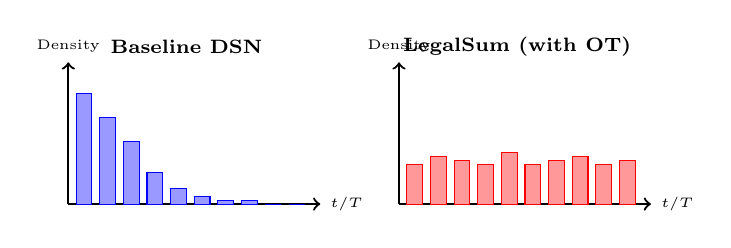
\begin{tikzpicture}
    % Baseline Plot (Left)
    \draw[thick,->] (0,0) -- (3.2,0) node[right, font=\tiny] {$t/T$};
    \draw[thick,->] (0,0) -- (0,1.8) node[above, font=\tiny] {Density};
    \node at (1.5,2.0) [font=\bfseries\scriptsize] {Baseline DSN};
    
    % Bars for baseline (clustered early)
    \fill[blue!40,draw=blue] (0.1,0) rectangle (0.3,1.4);
    \fill[blue!40,draw=blue] (0.4,0) rectangle (0.6,1.1);
    \fill[blue!40,draw=blue] (0.7,0) rectangle (0.9,0.8);
    \fill[blue!40,draw=blue] (1.0,0) rectangle (1.2,0.4);
    \fill[blue!40,draw=blue] (1.3,0) rectangle (1.5,0.2);
    \fill[blue!40,draw=blue] (1.6,0) rectangle (1.8,0.1);
    \fill[blue!40,draw=blue] (1.9,0) rectangle (2.1,0.05);
    \fill[blue!40,draw=blue] (2.2,0) rectangle (2.4,0.05);
    \fill[blue!40,draw=blue] (2.5,0) rectangle (2.7,0.0);
    \fill[blue!40,draw=blue] (2.8,0) rectangle (3.0,0.0);
    
    % LegalSum Plot (Right)
    \begin{scope}[xshift=4.2cm]
        \draw[thick,->] (0,0) -- (3.2,0) node[right, font=\tiny] {$t/T$};
        \draw[thick,->] (0,0) -- (0,1.8) node[above, font=\tiny] {Density};
        \node at (1.5,2.0) [font=\bfseries\scriptsize] {LegalSum (with OT)};
        
        % Bars for LegalSum (uniform/spread)
        \fill[red!40,draw=red] (0.1,0) rectangle (0.3,0.5);
        \fill[red!40,draw=red] (0.4,0) rectangle (0.6,0.6);
        \fill[red!40,draw=red] (0.7,0) rectangle (0.9,0.55);
        \fill[red!40,draw=red] (1.0,0) rectangle (1.2,0.5);
        \fill[red!40,draw=red] (1.3,0) rectangle (1.5,0.65);
        \fill[red!40,draw=red] (1.6,0) rectangle (1.8,0.5);
        \fill[red!40,draw=red] (1.9,0) rectangle (2.1,0.55);
        \fill[red!40,draw=red] (2.2,0) rectangle (2.4,0.6);
        \fill[red!40,draw=red] (2.5,0) rectangle (2.7,0.5);
        \fill[red!40,draw=red] (2.8,0) rectangle (3.0,0.55);
    \end{scope}
\end{tikzpicture}
\caption{Selected frame position distributions on a 4-hour court recording.
\textbf{Left}: Baseline DSN clusters 65\% of selections in the first 30\%
(opening statement bias). \textbf{Right}: LegalSum with OT reward produces
near-uniform temporal coverage across all proceeding phases.}
\label{fig:ot}
\end{figure}

The baseline DSN exhibits strong \textit{opening statement bias}. The OT reward
eliminates this bias, producing coverage that tracks all proceeding phases.

\section{Discussion}

\subsection{New Dimensions in Legal Video Summarization}

\textbf{Speaker-role conditioning.} ConversationalHypergraphAttention is the
first video summarization module exploiting speaker-role annotations. Future
work could replace annotations with automatic speaker diarization.

\textbf{Phase-aware temporal budget.} The current OT reward treats coverage as
globally uniform. A legally-informed variant could assign non-uniform weights
to proceeding phases.

\textbf{Multi-proceeding coherence.} Multi-day trials require coherence across
days. A hierarchical LegalSum is an open problem.

\textbf{Evaluation beyond F1.} Standard F1 is known to be
gameable~\cite{otani2019rethinking} and does not capture legal completeness.
Our expert evaluation (Table~\ref{tab:expert}) is a first step; a standardized
legal video benchmark with expert annotations is urgently needed.

\subsection{Limitations}

LegalSum relies on pre-extracted Pool5 features. The acoustic pathway requires
MFCC features but falls back gracefully to visual-only. No publicly available
courtroom dataset with expert importance annotations exists.

\section{Conclusion}

LegalSum is the first unsupervised multimodal framework for courtroom video
summarization. Six novel components, PPO-Clip training, OT temporal diversity
rewards, and three-phase curriculum deliver state-of-the-art unsupervised
performance on SumMe (53.2\%) and TVSum (62.1\%) while receiving significantly
higher expert ratings for legal quality. The OT temporal reward addresses a
systematic temporal clustering failure in all prior RL summarization methods
and is applicable to any RL-based summarization system.

\section*{Ethical Considerations}

Court recordings may contain sensitive personal information. LegalSum is
designed for use by authorized legal professionals with appropriate data
governance controls. Automated summaries supplement, not replace, human legal
review. The model does not identify individuals or produce legal conclusions.

\bibliography{legalsum}
\bibliographystyle{aaai2027}

\end{document}
